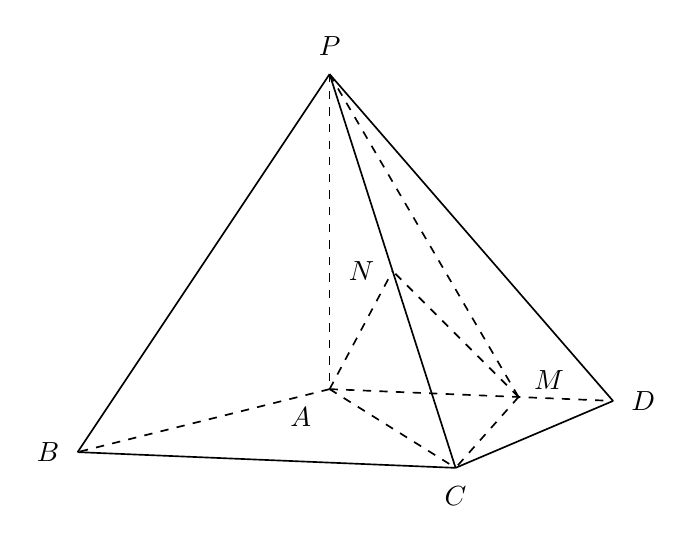
\begin{tikzpicture}[x=1cm,y=1cm,line width=.6pt,font=\normalsize]
\coordinate (P) at (0.0000000000,5.2000000000);
\coordinate (A) at (0.0,1.2);
\coordinate (B) at (-3.2,0.4);
\coordinate (C) at (1.6,0.2);
\coordinate (D) at (3.6000000000,1.0500000000);
\coordinate (M) at (2.4000000000,1.1000000000);
\coordinate (N) at (0.8000000000,2.7000000000);
% solid visible edges
\draw[solid] (P)--(B);
\draw[solid] (P)--(C);
\draw[solid] (P)--(D);
\draw[solid] (B)--(C);
\draw[solid] (C)--(D);
% dashed hidden / interior edges
\draw[dashed] (P)--(A);
\draw[dashed] (A)--(B);
\draw[dashed] (A)--(D);
\draw[dashed] (A)--(C);
\draw[dashed] (P)--(M);
\draw[dashed] (A)--(N);
\draw[dashed] (M)--(C);
\draw[dashed] (M)--(N);
\node[above,yshift=3.0pt] at (P) {$P$};
\node[below left,xshift=-3pt,yshift=-3.0pt] at (A) {$A$};
\node[left,xshift=-3pt] at (B) {$B$};
\node[below,yshift=-3pt] at (C) {$C$};
\node[right,xshift=3pt] at (D) {$D$};
\node[right,xshift=2pt,yshift=6pt] at (M) {$M$};
\node[left,xshift=-3pt] at (N) {$N$};
\end{tikzpicture}